% !TeX root = paper.tex
\section{Experiment: Elementary Perceptual Tasks}

Cleveland and McGill describe a set of elementary graphical perceptual tasks across ten encodings, where each encodes a quantitative variable in a graphical element or visual mark~\cite{cleveland_mcgill,cleveland1985graphical}. These tasks are the low-level building blocks for information visualizations (Table~\ref{tab:encoding_parameters}): estimating position on a common scale, position on non-aligned scales, length, direction (or slope), angle, area, volume, curvature,  shading (or ink density), and color saturation. As human color perception is complex, and because Cleveland and McGill perform no experiments with it, for now we leave it for future work. 

For the remaining nine tasks, we create visualizations as 100$\times$100 raster images, and test whether each of our networks is able to regress values from the images. As discussed in Section~\ref{sec:measuresandanalysis}, we generate multiple parameterizations for each elementary perceptual task to allow us to increase the number of parameters that the networks must estimate, and to measure performance as we move closer towards a general representation of visual marks. For instance, for \emph{Position Common Scale}, first we only vary the $y$-position of the spot to estimate against the scale, then we include translation along the x-axis, and then we vary the size of the spot size. These parameterizations are still simple---each increase is only slightly more complex for a human to solve---but it rapidly increases the number of possible images that the network must `learn' (Table~\ref{tab:encoding_parameters}).

JT: Write something about comparison to Cleveland and McGill's 1985 experimental encoding?

JT: Write something more intelligent about the different kinds of parameter variations.

%Cleveland and McGill did not explicitly test human perception of single instances of these encodings. -> JT: We now know this isn't true.

%\begin{figure}[t]
%	  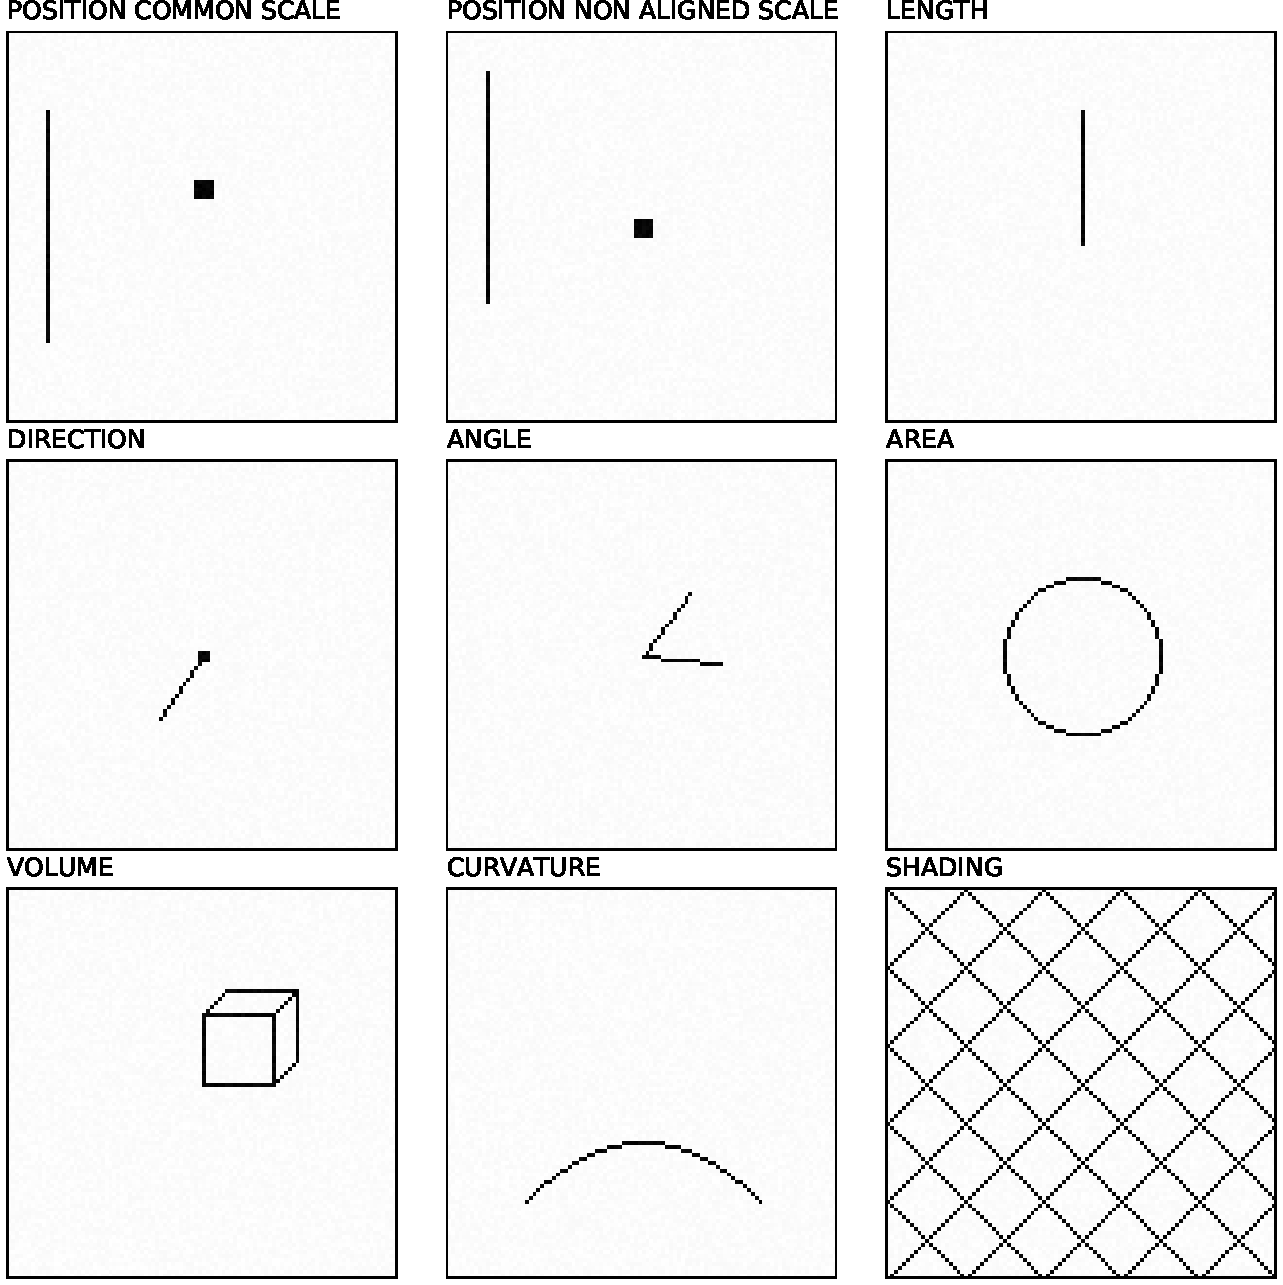
\includegraphics[width=\linewidth]{figure1_overview.pdf}
%  \caption{\textbf{Elementary Perceptual Tasks.} Rasterized visualizations of the elementary perceptual tasks as defined by Cleveland and McGill~\cite{cleveland_mcgill} (color saturation excluded). We vary the parameters of each perceptual task and then assess the interpretability of feed-forward neural networks.}
%	\label{fig:elementary_perceptual_tasks}
%\end{figure}



\begin{table}[!ht]
\centering
\caption{\textbf{Elementary Perceptual Tasks.} Rasterized visualizations of the elementary perceptual tasks as defined by Cleveland and McGill~\cite{cleveland_mcgill} (color saturation excluded). We sequentially increase the number of parameters for every task (e.g., by adding translation). This introduces variability and creates increasingly more complex datasets.}
\resizebox{\linewidth}{!}{
\begin{tabular}{lllr}
	\toprule
	\multicolumn{2}{l}{Elementary Perceptual Task} & ~ & Permutations\\
	\midrule
	\raisebox{-.85\height}{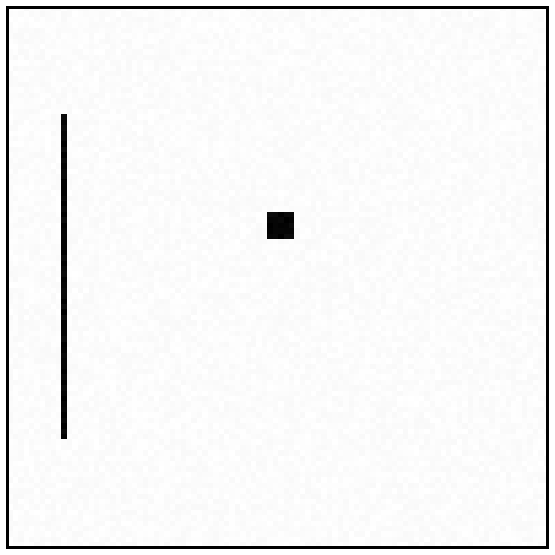
\includegraphics[width=.5in]{position_common_scale.pdf}} & \makecell[tl]{\emph{Position Common Scale}\\~~~Position Y\\~~~+ Position X \\~~~+ Spot Size \\} &~& \makecell[tr]{~\\ $60$ \\ $3,600$ \\ $216,00$}\\

	\midrule
	\raisebox{-.85\height}{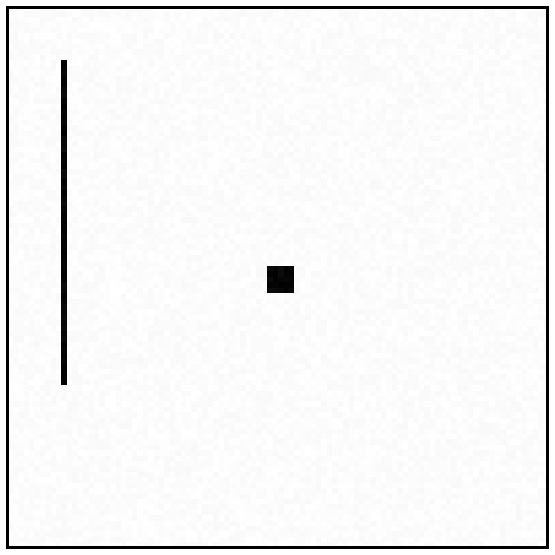
\includegraphics[width=.5in]{position_non_aligned_scale.pdf}} & \makecell[tl]{\emph{Position Non-Aligned Scale}\\~~~Position Y\\~~~+ Position X \\~~~+ Spot Size \\} &~& \makecell[tr]{~\\ $600$ \\ $36,000$ \\ $216,000$}\\

	\midrule
	\raisebox{-.95\height}{
\includegraphics[width=.5in]{length.pdf}} & \makecell[tl]{\emph{Length}\\~~~Length\\~~~+ Position Y \\~~~+ Position X \\~~~+ Width} &~& \makecell[tr]{ ~\\$60$ \\ $2,400$ \\ $144,000$\\$864,000$}\\

	\midrule
	\raisebox{-.85\height}{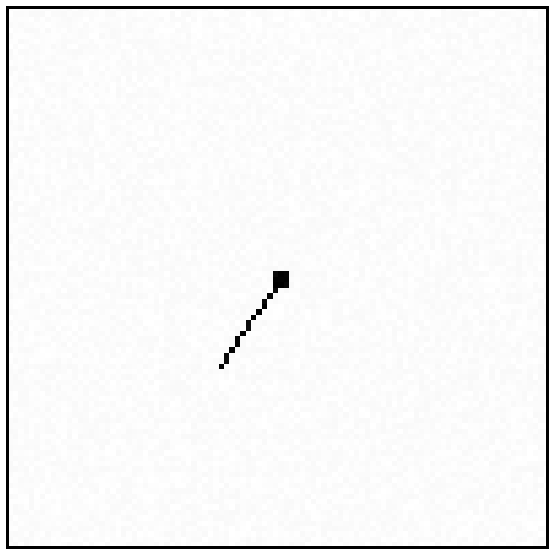
\includegraphics[width=.5in]{direction.pdf}} & \makecell[tl]{\emph{Direction}\\~~~Angle\\~~~+ Position Y \\~~~+ Position X} &~& \makecell[tr]{ ~\\$360$ \\ $21,600$ \\ $1,296,000$}\\

	\midrule
	\raisebox{-.85\height}{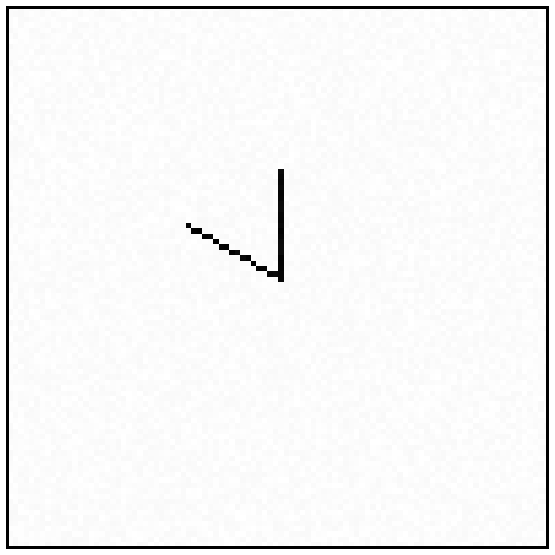
\includegraphics[width=.5in]{angle.pdf}} & \makecell[tl]{\emph{Angle}\\~~~Angle\\~~~+ Position Y \\~~~+ Position X} &~& \makecell[tr]{ ~\\$90$ \\ $5,400$ \\ $324,000$}\\

	\midrule
	\raisebox{-.85\height}{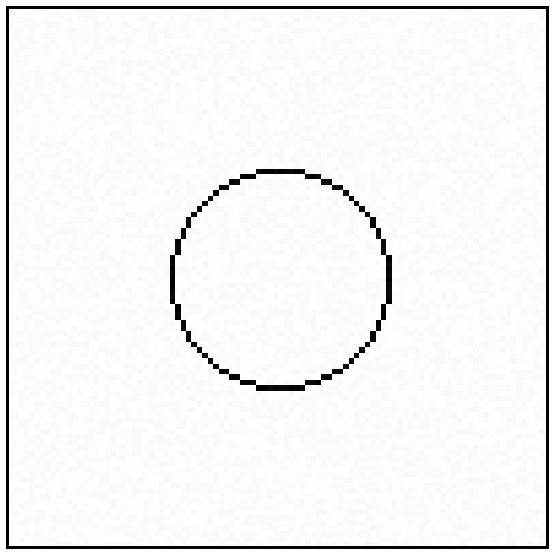
\includegraphics[width=.5in]{area.pdf}} & \makecell[tl]{\emph{Area}\\~~~Radius\\~~~+ Position Y \\~~~+ Position X} &~& \makecell[tr]{ ~\\$40$ \\ $800$ \\ $16,000$}\\

	\midrule
	\raisebox{-.85\height}{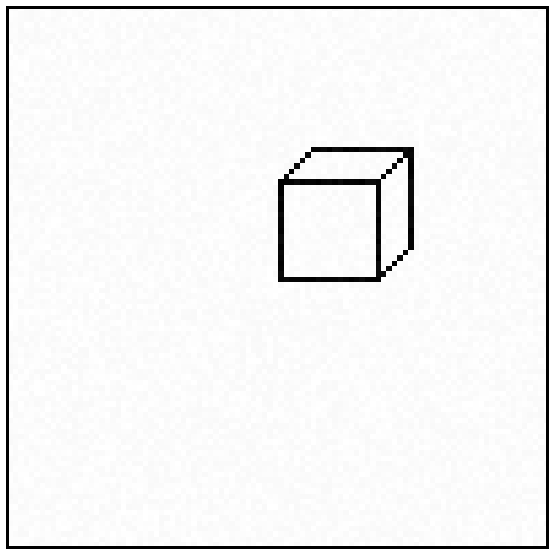
\includegraphics[width=.5in]{volume.pdf}} & \makecell[tl]{\emph{Volume}\\~~~Cube Sidelength\\~~~+ Position Y \\~~~+ Position X} &~& \makecell[tr]{ ~\\$20$ \\ $400$ \\ $8,000$}\\
	
	\midrule
	\raisebox{-.85\height}{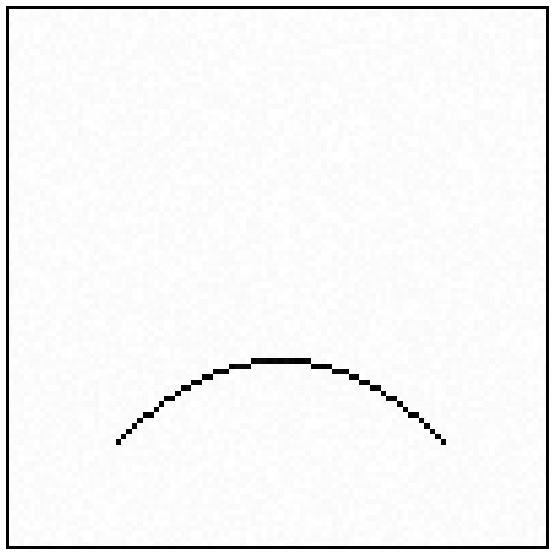
\includegraphics[width=.5in]{curvature.pdf}} & \makecell[tl]{\emph{Curvature}\\~~~Midpoint Curvature\\~~~+ Position Y \\~~~+ Position X} &~& \makecell[tr]{ ~\\$80$ \\ $1,600$ \\ $64,000$}\\	

	\midrule
	\raisebox{-.85\height}{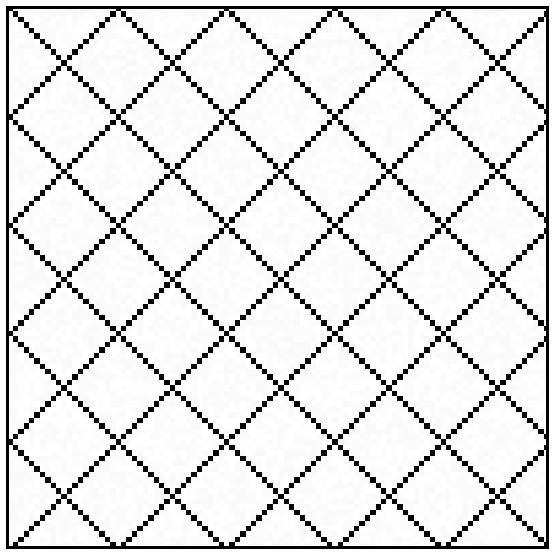
\includegraphics[width=.5in]{shading.pdf}} & \makecell[tl]{\emph{Shading}\\~~~Density\\~~~+ Position Y \\~~~+ Position X} &~& \makecell[tr]{ ~\\$100$ \\ $2,000$ \\ $40,000$}\\	
%	
	\bottomrule
\end{tabular}
}
\label{tab:encoding_parameters}
\end{table}



%
\subsection{Hypotheses}

We state four hypotheses for the elementary perceptual task experiment:

\begin{itemize}
	\item \textbf{H1.1} \textbf{The CNNs tested will be able to regress quantitative variables from graphical elements.} We parametrize different visual encodings (Table~\ref{tab:encoding_parameters}) and test whether the CNNs can measure them, and relate the results to accuracies obtained by humans on similar tasks.
	\item \textbf{H1.2} \textbf{Computed perceptual performance is dependent on network architexture.} We evaluate multiple regressors with different numbers of trainable parameters. We expect a more complex network (with a higher number of trainable parameters) to perform better on elementary perceptual tasks.
	\item \textbf{H1.3} \textbf{Some visual encodings will be easier to learn than others for the CNNs tested.} Cleveland and McGill order the elementary perceptual tasks by accuracy. We investigate whether this order is also relevant for computing graphical perception.
	\item \textbf{H1.4} \textbf{Networks trained on perceptual tasks can generalize to more and less complex variations of the same task.} Empirical evidence suggests that CNNs are able to generalize by interpolating between different training data points. This property allows them to perform on variations of a similar perceptual task. We create visual representations of the elementary perceptual tasks with different variability, and expect that networks will be able to generalize when presented with slight task variations.
\end{itemize}

%	
%	We suspect that CNNs are able to 'learn` absolute quantities encoded using low-level visual 
%	
%	While much simpler models than their biological pendant, convolutional neural networks are heavily influenced by our biological knowledge of the visual system. Such classifiers therefor follow the same principles as human perception.


\subsection{Results}

%While the performance varies for the different encodings, we observe for all networks performance similar to the measured human performance by Cleveland and McGill~\cite{cleveland1985graphical}. These results confirm our initial hypotheses.
\noindent{\textbf{Overall Accuracy.}} The tested CNNs and MLP are able to regress the visually encoded quantities in most cases (Fig.~\ref{fig:figure1_results}), with average error across all classifiers and tasks as \textit{MLAE}$=1.597$ ($SD=0.394$). % and \textit{MAE}=$2.89$ ($SD=0.848$). 
These values are similar or better than the range of MLAE=$3.02$--$3.82$ ($8-14\%$ error) for a similar experiment by Cleveland and McGill testing human estimation of relations between elementary perceptual tasks~\cite{cleveland1985graphical}. From these results, we \textbf{accept H1.1}.
\\~\\
\noindent{\textbf{Comparing Networks.}} 
Across network architectures and training schemes, there is considerable difference in performance. In order of decreasing error: 
The MLP has \textit{MLAE}$=2.943$ ($SD=0.857$), 
for LeNet $2.125$ ($SD=0.38$), 
Xception trained on ImageNet $1.627$ ($SD=0.462$), 
Xception trained from scratch $1.504$ ($SD=0.493$),
VGG19 trained on ImageNet $0.979$ ($SD=0.581$), 
and VGG19 trained from scratch $0.404$ ($SD=0.407$).

Across tasks, we compare the average regression performances for our networks and report the effect of the network as statistically significant ($F_{5,48}=20.392,p<0.01$). Post hoc comparisons show that the differences between LeNet and the VGG19 network, independent of the used weights, are significant ($t_48=4.674,p<0.01$). VGG19 from scratch and Xception (both versions) perform significantly differently, with Xception from scratch ($t_48=4.87,p<0.01$) and Xception with ImageNet weights ($t_48=5.621,p<0.01$). However, differences between LeNet and both Xception networks are not significant. Taken collectively, we \textbf{partially accept H1.2}, in that more tunable parameters does not automatically infer greater performance.
\\~\\
\noindent{\textbf{Ranking of Visual Encodings.}} Cleveland and McGill provide an ordering of elementary visual encodings based on theoretical arguments and experimental results. We compare their ranking with rankings of our networks in Table~\ref{tab:ranking}. We note that the rankings between networks using ImageNet weights is identical; however, overall, there is significant variability, and we \textbf{reject H1.3}. 

%Observing Figure~\ref{fig:figure1_results}, -> JT: we should do this.

%Since such a ranking see,s to heavily depend on the used regressor, the weights, and the initialization, we do not think a generalized ranking can be created and \textbf{reject H1.3}.

\begin{table}[tb]
\centering
\caption{\textbf{Ranking of Elementary Perceptual Tasks.} We create a ranking of the elementary perceptual tasks for all of our networks. We report midmean logistic absolute errors (MLAE) for each network averaged across multiple runs on the most complex parametrization of the individual stimuli. The VGG19 network performs best compared on all tasks. For human performance, we report the ranking of Cleveland and McGill~\cite{cleveland_mcgill}. The VGG19 * and Xception * networks use ImageNet weights and yield identical rankings.}
\resizebox{\linewidth}{!}{
\begin{tabular}{cllllll}
\toprule
Human (CMcG) & MLP & LeNet & VGG19 * & \textbf{VGG19} & Xception * & Xception \\
\midrule
\multicolumn{7}{l}{\emph{Position Common Scale}} \\
1. & 7. (3.84) & 2. (1.36) & 5. (1.02) & \textbf{3.} (-0.04) & 5. (1.65) & 1. (1.04)\\
\multicolumn{7}{l}{\emph{Position Non aligned Scale}} \\
2. & 6. (3.61) & 1. (1.35) & 6. (1.09) & \textbf{5.} (0.26) & 6. (1.71) & 2. (1.06)\\
\multicolumn{7}{l}{\emph{Length}} \\
3. & 1. (1.99) & 8. (3.19) & 4. (0.87) & \textbf{2.} (-0.14) & 4. (1.59) & 3. (1.11) \\
\multicolumn{7}{l}{\emph{Direction}} \\
3. & 9. (4.65) & 7. (3.07) & 9. (2.84) & \textbf{8.} (0.92) & 9. (3.46) & 6. (1.57) \\
\multicolumn{7}{l}{\emph{Angle}} \\
3. & 8. (4.61) & 9. (3.33) & 8. (2.31) & \textbf{9.} (0.99) & 8. (2.60) & 7. (1.72) \\
\multicolumn{7}{l}{\emph{Area}} \\
4. & 2. (2.01) & 5. (2.21) & 1. (0.49) & \textbf{1.} (-0.17) & 1. (0.80) & 5. (1.38) \\
\multicolumn{7}{l}{\emph{Volume}} \\
5. & 4. (2.38) & 4. (1.91) & 7. (1.16) & \textbf{7.} (0.87) & 7. (2.03) & 9. (2.10) \\
\multicolumn{7}{l}{\emph{Curvature}} \\
5. & 3. (2.34) & 3. (1.81) & 2. (0.71) & \textbf{6.} (0.28) & 2. (1.17) & 4. (1.13) \\
\multicolumn{7}{l}{\emph{Shading}} \\
6. & 5. (3.04) & 6. (2.23) & 3. (0.73) & \textbf{4.} (0.14) & 3. (1.57) & 8. (1.82) \\

% 
%\makecell[tl]{\emph{Position}\\~~\emph{Non-aligned Scale}} & 1 & 1 & 2 & 3 & \textbf{4} & 5 & 6 \\
%\makecell[tl]{\emph{Length}} & 1 & 1 & 2 & 3 & \textbf{4} & 5 & 6 \\
%\makecell[tl]{\emph{Direction}} & 1 & 1 & 2 & 3 & \textbf{4} & 5 & 6 \\
%\makecell[tl]{\emph{Angle}} & 1 & 1 & 2 & 3 & \textbf{4} & 5 & 6 \\
%\makecell[tl]{\emph{Area}} & 1 & 1 & 2 & 3 & \textbf{4} & 5 & 6 \\
%\makecell[tl]{\emph{Volume}} & 1 & 1 & 2 & 3 & \textbf{4} & 5 & 6 \\
%\makecell[tl]{\emph{Curvature}} & 1 & 1 & 2 & 3 & \textbf{4} & 5 & 6 \\
%\makecell[tl]{\emph{Shading}} & 1 & 1 & 2 & 3 & \textbf{4} & 5 & 6 \\
%\begin{tabular}{ll}
%	\toprule
%	Task & \begin{tabular}{ccccccc}
%			Human & MLP & LeNet & VGG19 * & VGG19 & Xception * & Xception
%			\end{tabular}\\
%	\midrule
%	\raisebox{-.85\height}{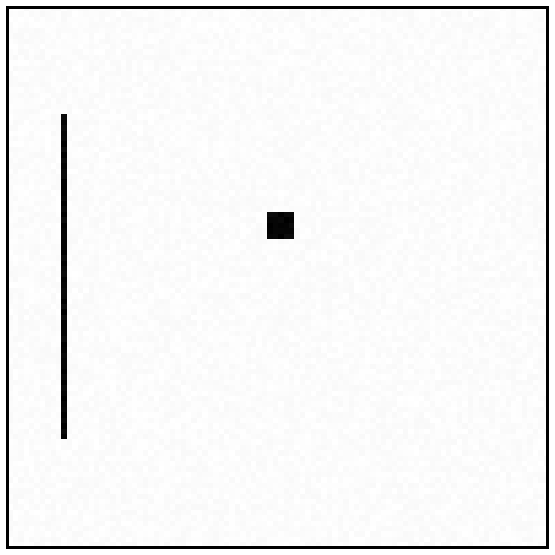
\includegraphics[width=.5in]{position_common_scale.pdf}} & \makecell[tl]{\emph{Position Common Scale}\\ \begin{tabular}{ccccccc}
%
%\end{tabular}} \\
%
%	\midrule
%	\raisebox{-.85\height}{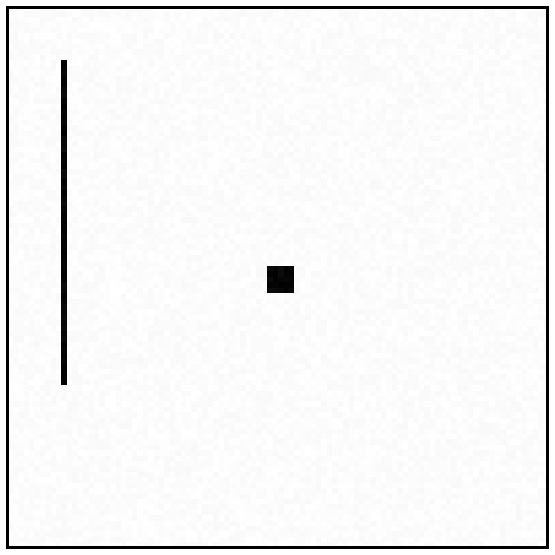
\includegraphics[width=.5in]{position_non_aligned_scale.pdf}} & \makecell[tl]{\emph{Position Non-Aligned Scale}\\~~~Position Y\\~~~+ Position X \\~~~+ Spot Size \\} &~& \makecell[tr]{~\\ $600$ \\ $36,000$ \\ $216,000$}\\
%
%	\midrule
%	\raisebox{-.95\height}{
\includegraphics[width=.5in]{length.pdf}} & \makecell[tl]{\emph{Length}\\~~~Length\\~~~+ Position Y \\~~~+ Position X \\~~~+ Width} &~& \makecell[tr]{ ~\\$60$ \\ $2,400$ \\ $144,000$\\$864,000$}\\
%
%	\midrule
%	\raisebox{-.85\height}{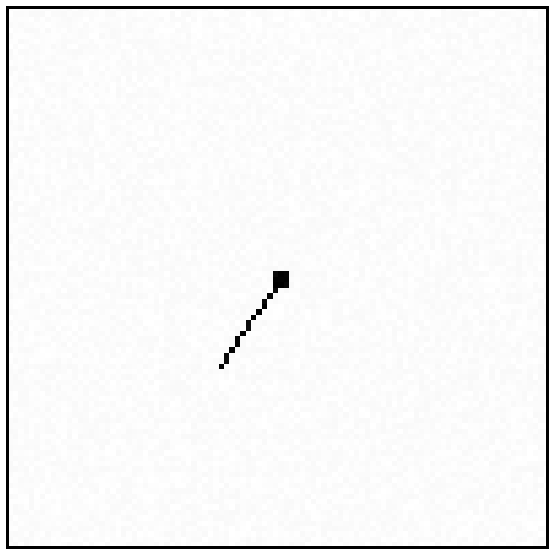
\includegraphics[width=.5in]{direction.pdf}} & \makecell[tl]{\emph{Direction}\\~~~Angle\\~~~+ Position Y \\~~~+ Position X} &~& \makecell[tr]{ ~\\$360$ \\ $21,600$ \\ $1,296,000$}\\
%
%	\midrule
%	\raisebox{-.85\height}{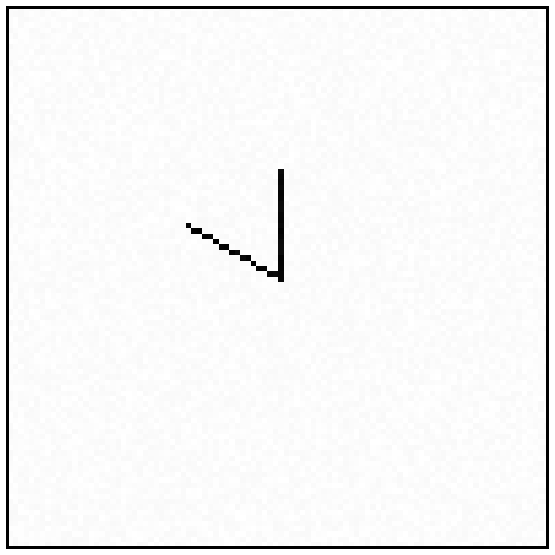
\includegraphics[width=.5in]{angle.pdf}} & \makecell[tl]{\emph{Angle}\\~~~Angle\\~~~+ Position Y \\~~~+ Position X} &~& \makecell[tr]{ ~\\$90$ \\ $5,400$ \\ $324,000$}\\
%
%	\midrule
%	\raisebox{-.85\height}{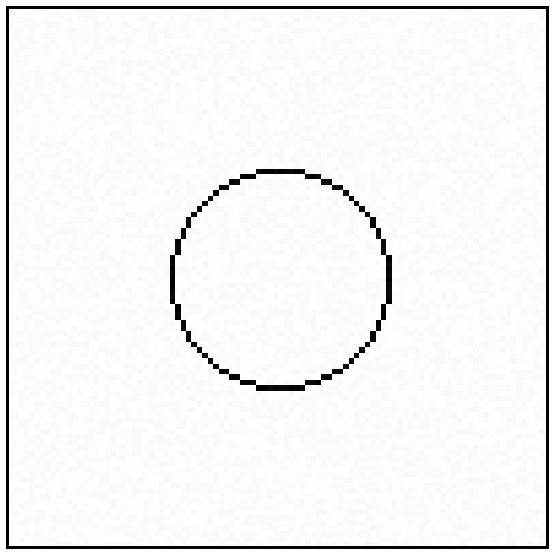
\includegraphics[width=.5in]{area.pdf}} & \makecell[tl]{\emph{Area}\\~~~Radius\\~~~+ Position Y \\~~~+ Position X} &~& \makecell[tr]{ ~\\$40$ \\ $800$ \\ $16,000$}\\
%
%	\midrule
%	\raisebox{-.85\height}{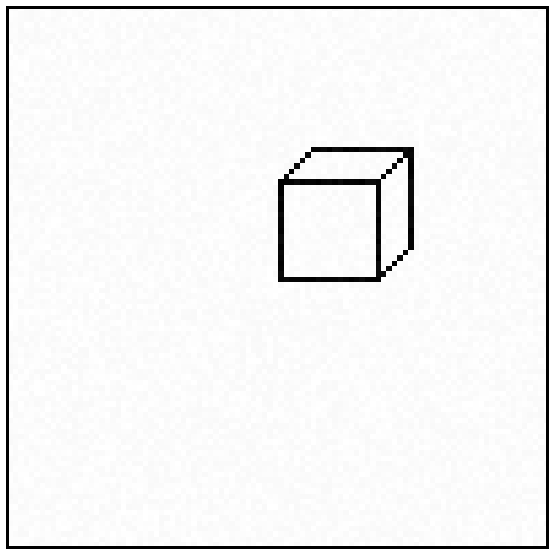
\includegraphics[width=.5in]{volume.pdf}} & \makecell[tl]{\emph{Volume}\\~~~Cube Sidelength\\~~~+ Position Y \\~~~+ Position X} &~& \makecell[tr]{ ~\\$20$ \\ $400$ \\ $8,000$}\\
%	
%	\midrule
%	\raisebox{-.85\height}{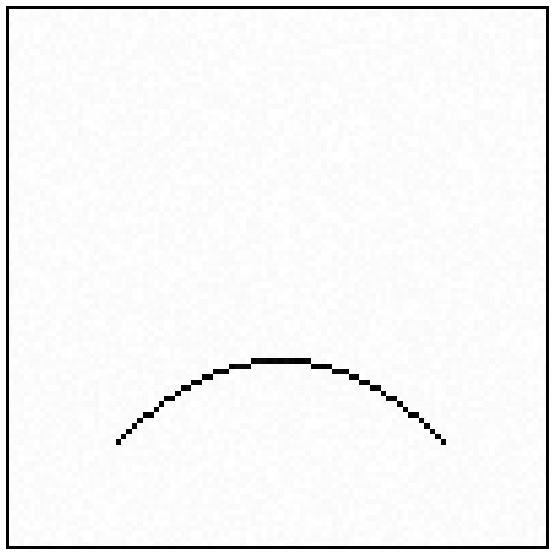
\includegraphics[width=.5in]{curvature.pdf}} & \makecell[tl]{\emph{Curvature}\\~~~Midpoint Curvature\\~~~+ Position Y \\~~~+ Position X} &~& \makecell[tr]{ ~\\$80$ \\ $1,600$ \\ $64,000$}\\	
%
%	\midrule
%	\raisebox{-.85\height}{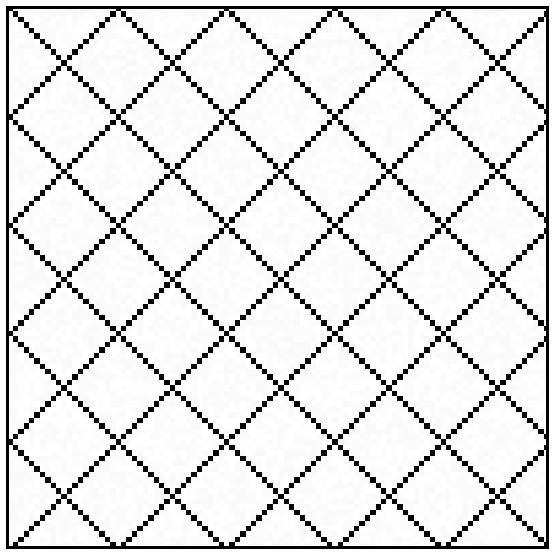
\includegraphics[width=.5in]{shading.pdf}} & \makecell[tl]{\emph{Shading}\\~~~Density\\~~~+ Position Y \\~~~+ Position X} &~& \makecell[tr]{ ~\\$100$ \\ $2,000$ \\ $40,000$}\\	

	\bottomrule
\end{tabular}
}
\label{tab:ranking}
\end{table}

\begin{figure}[!ht]
	\centering
	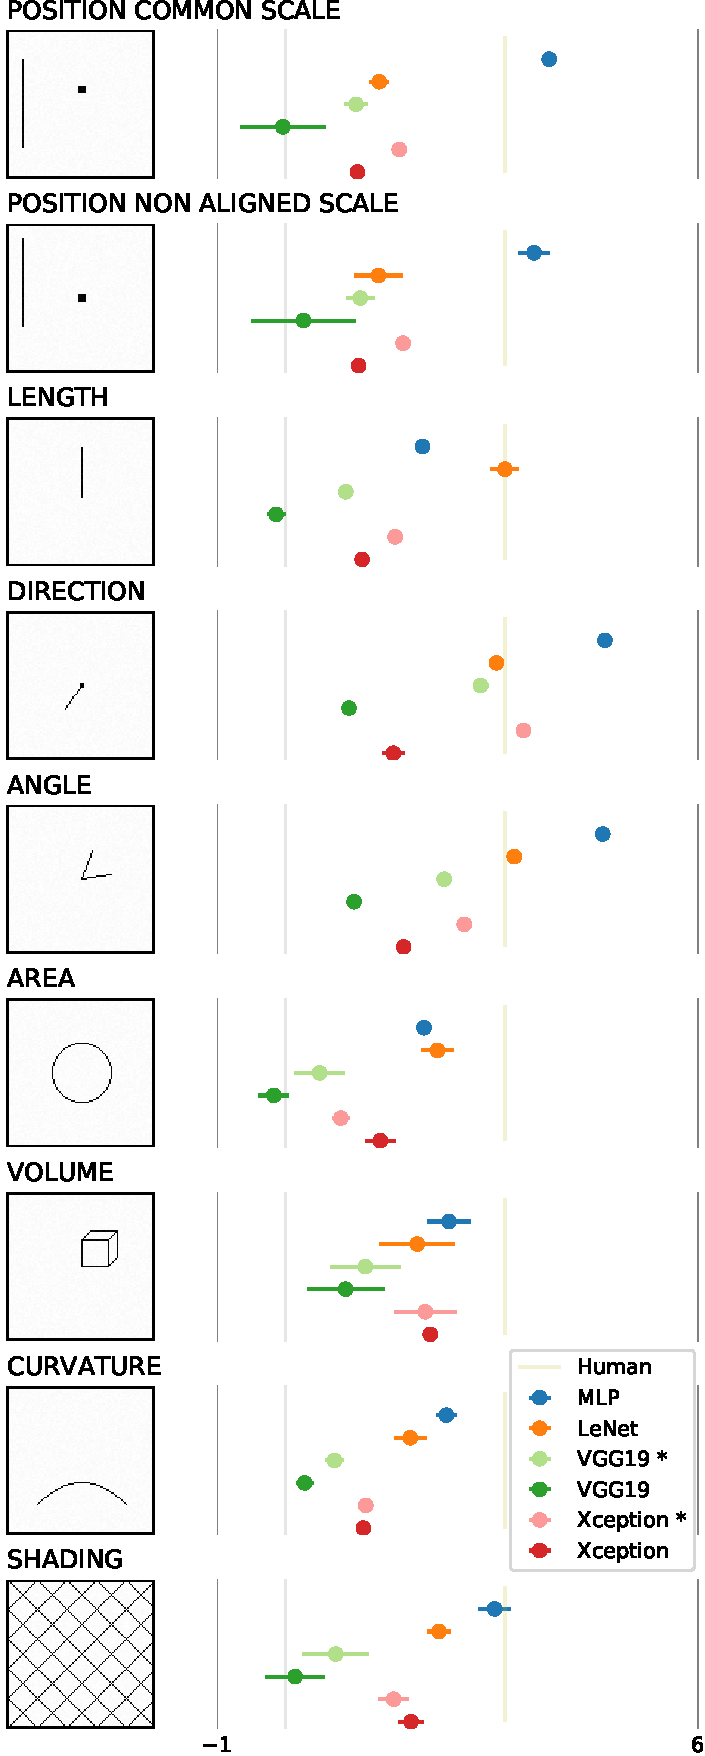
\includegraphics[width=.8\linewidth]{figure1_slim_only_last.pdf}
%	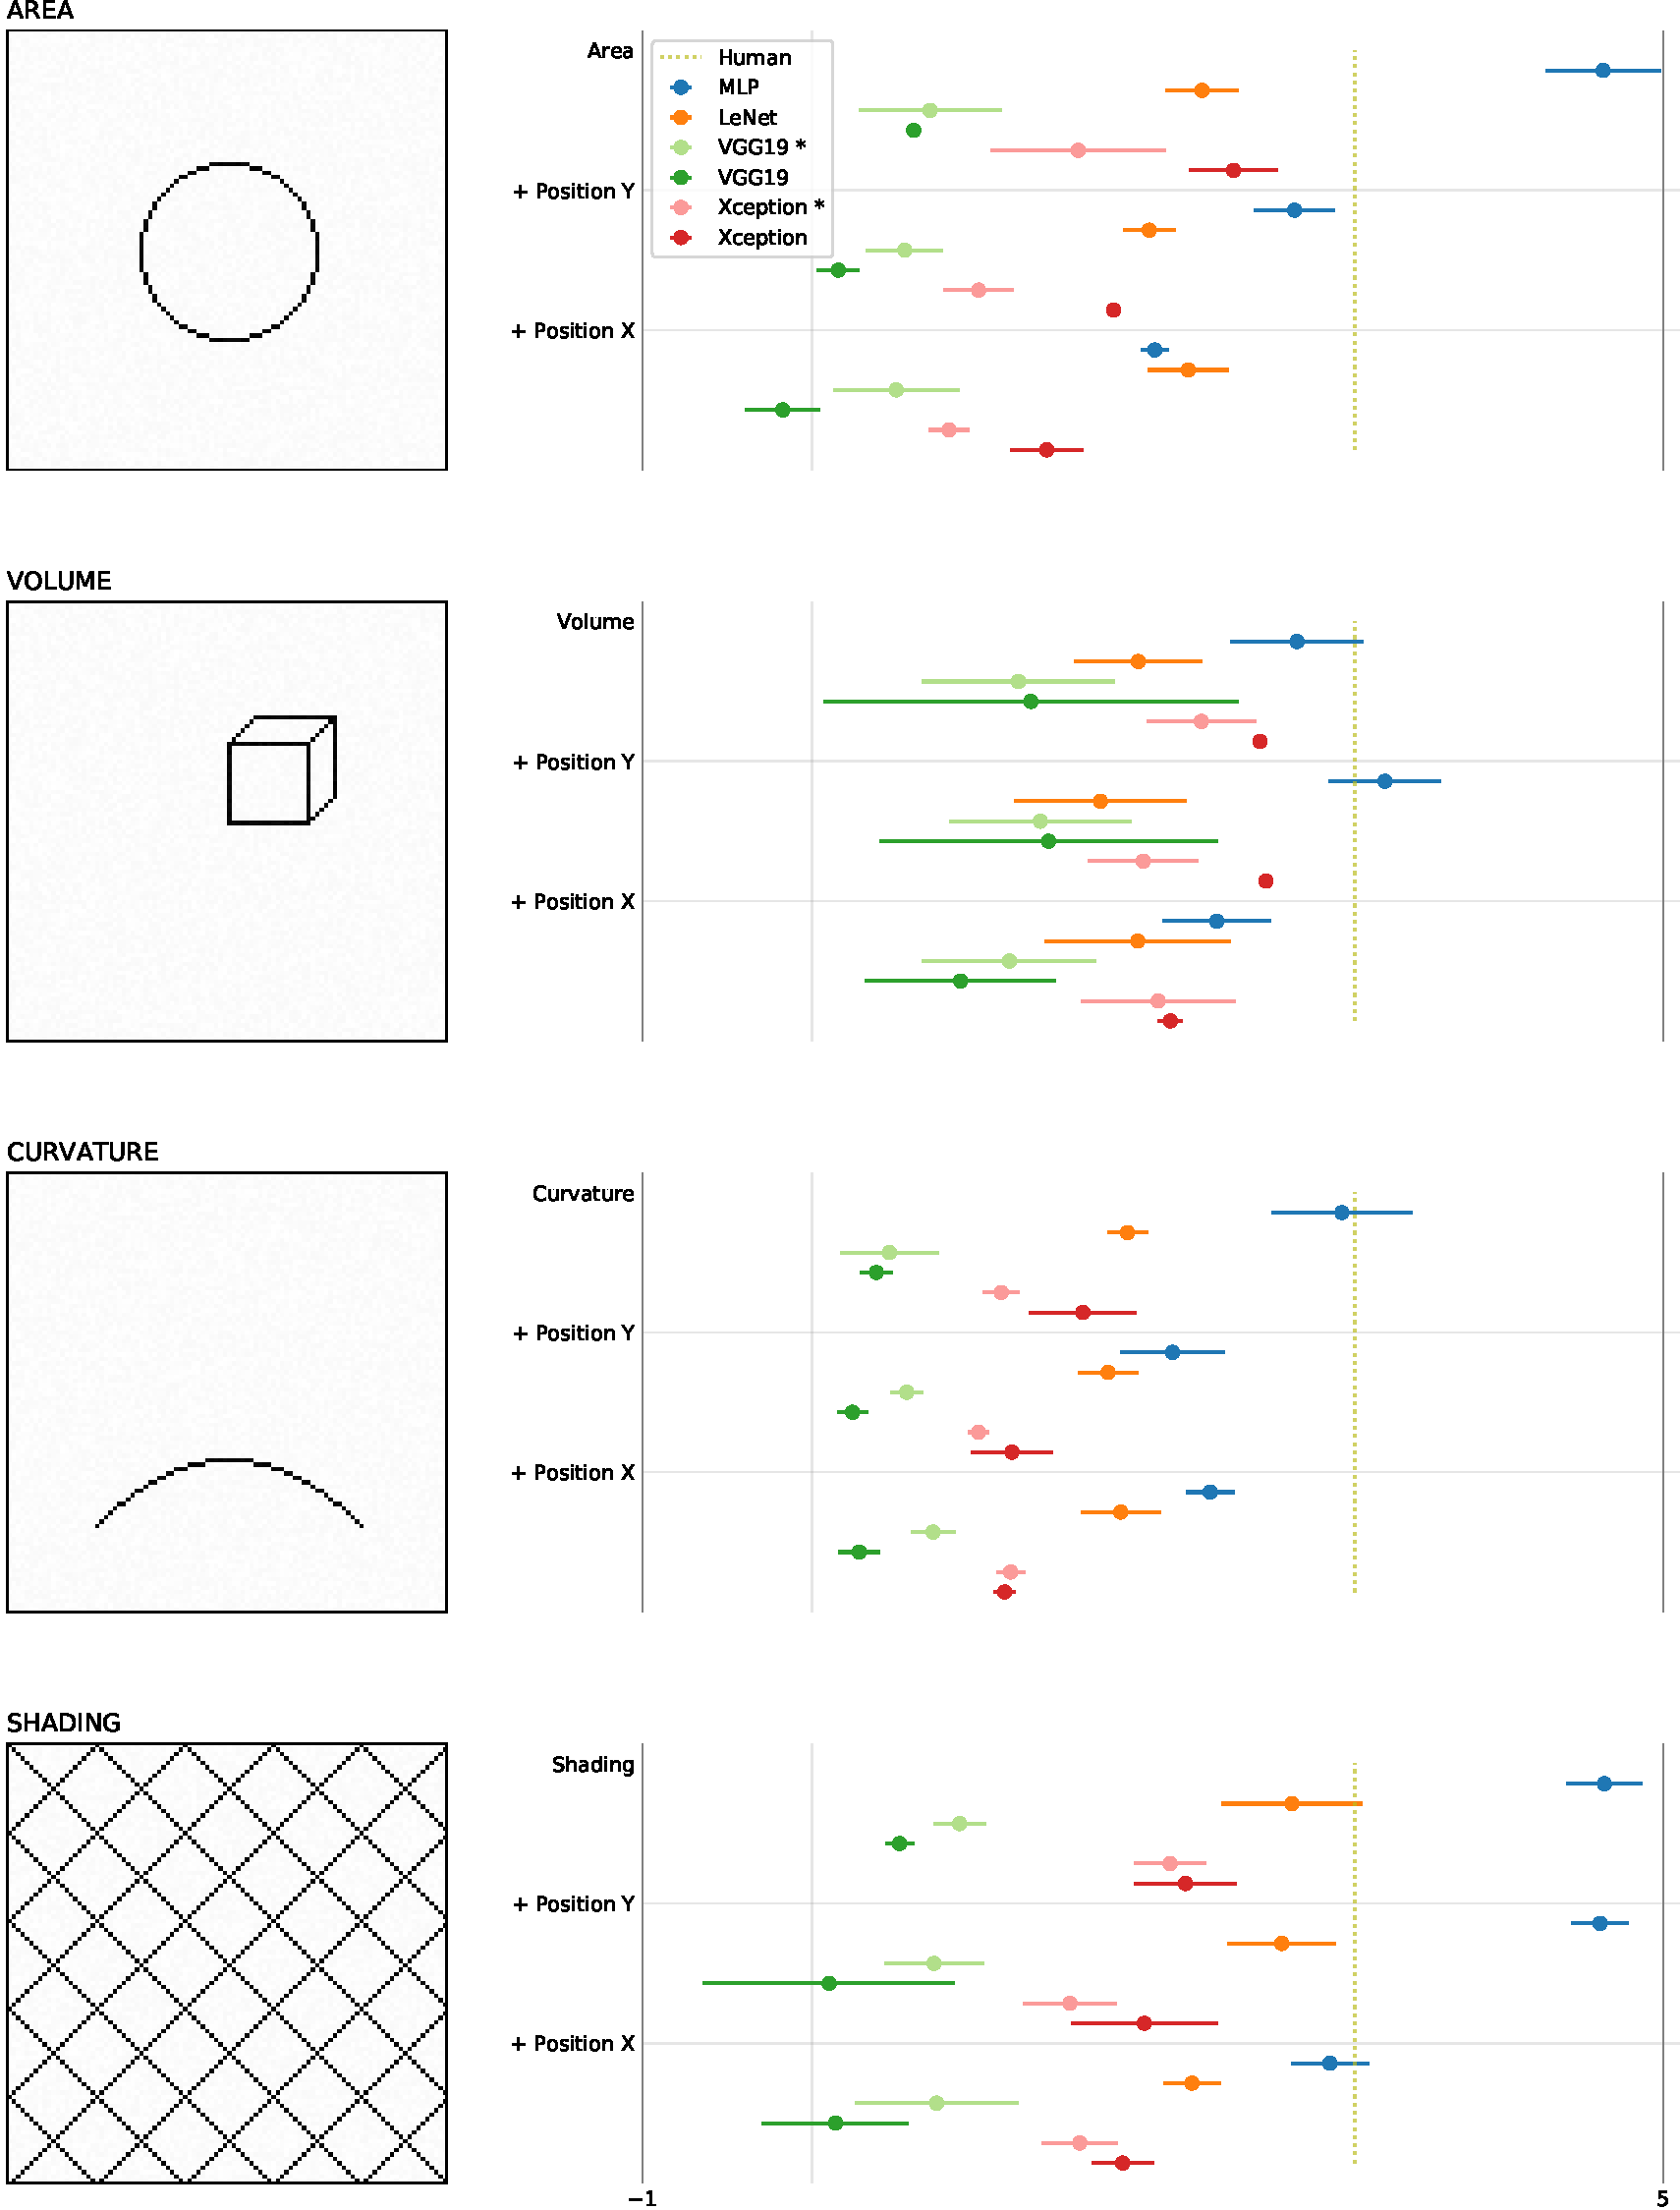
\includegraphics[width=0.48\linewidth]{figure1_slim_right.pdf}
	\caption{\textbf{Elementary perceptual tasks results for most complex task parameterization.} \emph{Left:} Example stimuli image. \emph{Right:} MLAE and 95\% confidence intervals for different networks. The * indicates networks which use ImageNet weights up until the MLP, rather than being trained from scratch.}
	\label{fig:figure1_results}
\end{figure}

\noindent{\textbf{Cross-classifier Variability and Network Generalizability.}} We measure regression performance across classifiers trained on the different parameterizations of the elementary perceptual tasks. Looking at the results in Fig.~\ref{fig:cross_network}, we can observe that even slight variations of an encoding such as added translation in Y or X drastically increases the error. We think that the networks are not really learning concepts of perception but rather learn the variation of pixel values.

\begin{figure}[!ht]
	\centering
	  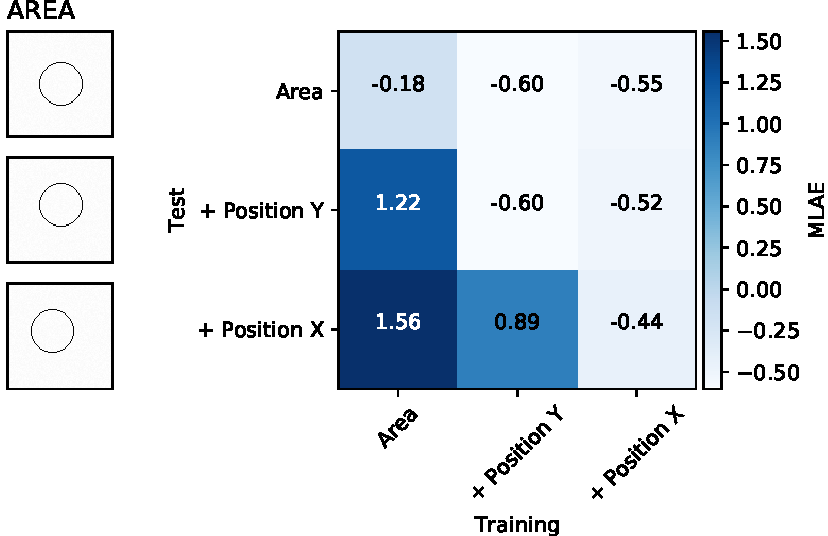
\includegraphics[width=.75\linewidth]{cross_network_small_VGG19_area.pdf}
	  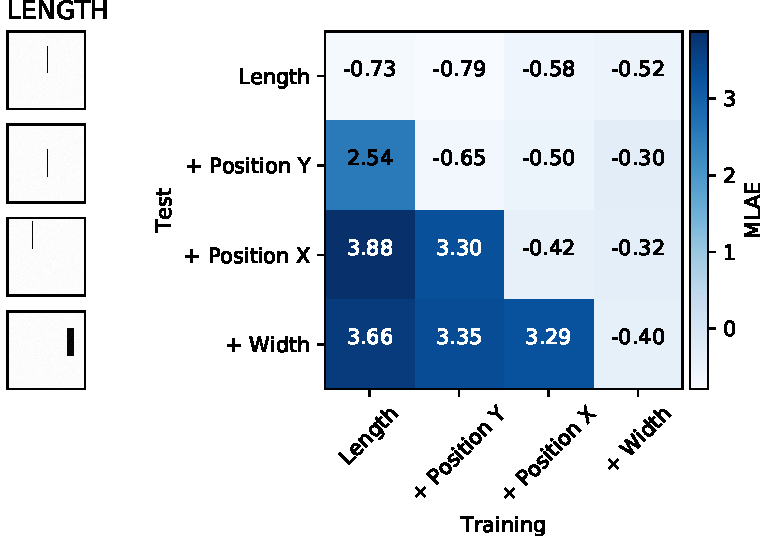
\includegraphics[width=.75\linewidth]{cross_network_small_VGG19_length.pdf}
	  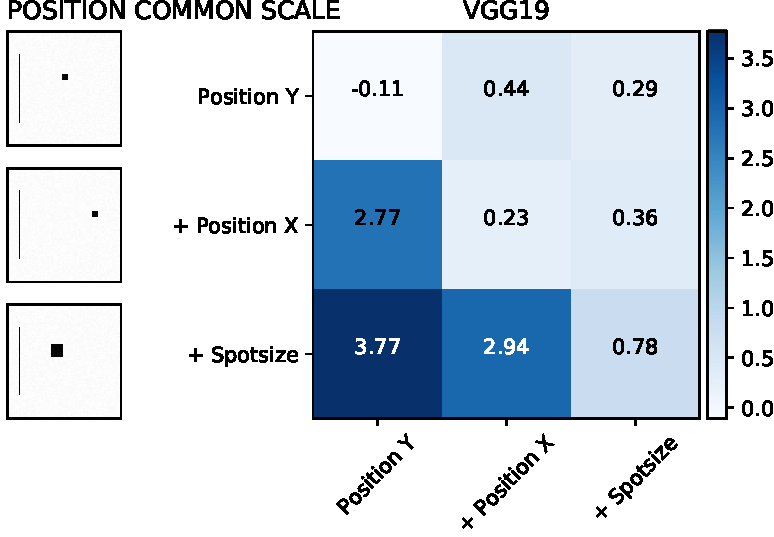
\includegraphics[width=.75\linewidth]{cross_network_small_VGG19_position_common_scale.pdf}
	  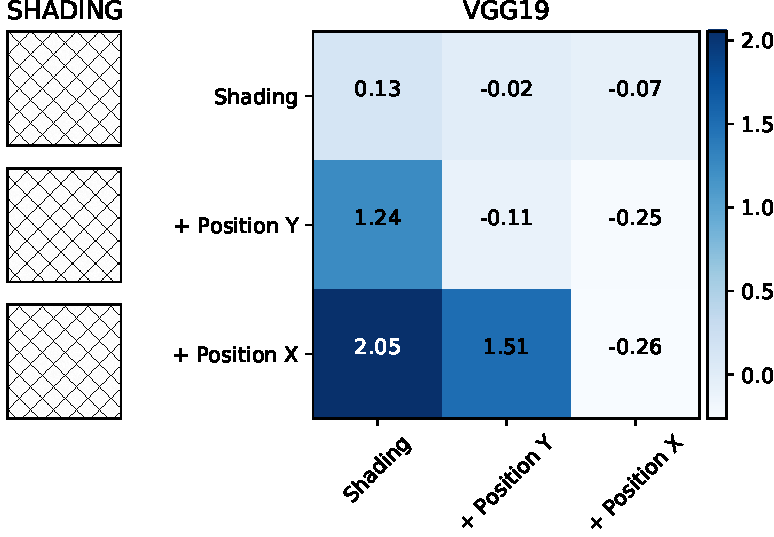
\includegraphics[width=.75\linewidth]{cross_network_small_VGG19_shading.pdf}
  \caption{\textbf{Cross-classifier variability for perceptual tasks.} We use predictions of the VGG19 network trained on different parametrizations of \emph{area}, \emph{length}, \emph{position common scale}, and \emph{shading}. These are the top 4 encodings in the ranking for this network. We measure the mean logistic absolute error (MLAE) -- the lower score, the better. Regressors trained on stimuli with variable position can generalize even if the axis of translation varies. However, if they are trained on fixed positions of the stimuli they are not able to measure translated encodings.}
	\label{fig:cross_network}
\end{figure}

